%【紙面設定】
%b4,横書き,2段
\documentclass[paper=b4j,landscape,twocolumn,fleqn]{jlreq}
\special{papersize=\the\paperwidth,\the\paperheight}
\setlength{\columnseprule}{0.4pt}
\pagestyle{empty}
\usepackage[margin=8truemm]{geometry}
\usepackage[dvipdfmx]{graphicx}
\usepackage{amsmath}
\usepackage{tikz}
\ModifyHeading{section}{lines=1,before_space=6pt,after_space=0pt}
\setlength{\parskip}{0pt}
\setlength{\jot}{3pt}

%【本文】
\begin{document}
\normalsize

\section{成分表示と大きさ 解答}
\begin{align*}
&1.\ 5\\[0.45em]
&2.\ 13\\[0.45em]
&3.\ \hat{c}=\begin{pmatrix}\frac35 & \frac45\end{pmatrix}\\[0.45em]
&4.\ \hat{d}=\begin{pmatrix}-\frac45 & \frac35\end{pmatrix}\\[0.45em]
&5.\ \begin{pmatrix}3 & 4\end{pmatrix}\\[0.45em]
&6.\ x^2+y^2=100
\end{align*}
\textbf{考え方}\
大きさは $|\vec{v}|=\sqrt{x^2+y^2}$ を使う。単位ベクトルは元のベクトルをその長さで割ればよい。\\
\textbf{図説（成分と単位ベクトル）}
\begin{center}
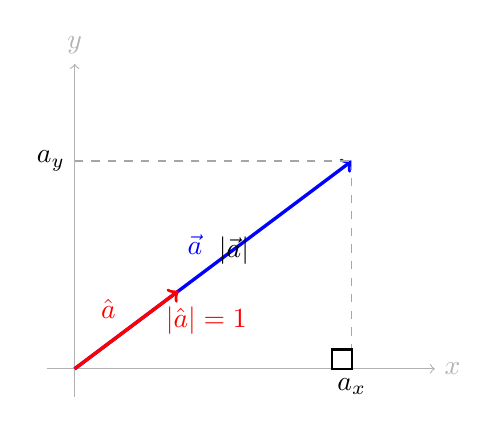
\begin{tikzpicture}[scale=0.88]
	\draw[->,gray!60] (-0.4,0) -- (5.2,0) node[right] {$x$};
	\draw[->,gray!60] (0,-0.4) -- (0,4.4) node[above] {$y$};
	\draw[very thick,blue,->] (0,0) -- (4,3) node[midway,above left] {$\vec{a}$};
	\draw[dashed,gray!70] (4,0) -- (4,3);
	\draw[dashed,gray!70] (0,3) -- (4,3);
	\draw[thick,black] (3.72,0) rectangle (4,0.28);
	\node[below] at (4,0) {$a_x$};
	\node[left] at (0,3) {$a_y$};
	\node at (2.3,1.7) {$|\vec{a}|$};
	\draw[very thick,red,->] (0,0) -- (1.5,1.125) node[midway,above left] {$\hat{a}$};
	\node[red] at (1.9,0.7) {$|\hat{a}|=1$};
\end{tikzpicture}
\end{center}
\textbf{途中式（代表例）}
\begin{align*}
&3.\ |\vec{c}|=\sqrt{6^2+8^2}=10,\ \hat{c}=\frac{1}{10}\begin{pmatrix}6 & 8\end{pmatrix}=\begin{pmatrix}\frac35 & \frac45\end{pmatrix}\\
&4.\ |\vec{d}|=\sqrt{(-4)^2+3^2}=5,\ \hat{d}=\frac{1}{5}\begin{pmatrix}-4 & 3\end{pmatrix}=\begin{pmatrix}-\frac45 & \frac35\end{pmatrix}\\
&6.\ |\vec{v}|=10\Rightarrow \sqrt{x^2+y^2}=10\Rightarrow x^2+y^2=100
\end{align*}

\newpage
\section{点と点を結ぶベクトル 解答}
\begin{align*}
&1.\ \overrightarrow{AB}=\begin{pmatrix}4 & 5\end{pmatrix},\ |\overrightarrow{AB}|=\sqrt{41}\\[0.45em]
&2.\ \overrightarrow{AB}=\begin{pmatrix}5 & -6\end{pmatrix},\ |\overrightarrow{AB}|=\sqrt{61}\\[0.45em]
&3.\ \overrightarrow{AB}=\begin{pmatrix}-6 & 8\end{pmatrix},\ |\overrightarrow{AB}|=10\\[0.45em]
&4.\ \overrightarrow{AB}=\begin{pmatrix}-6 & 6\end{pmatrix},\ |\overrightarrow{AB}|=6\sqrt{2}\\[0.45em]
&5.\ \overrightarrow{AB}=\begin{pmatrix}0 & -8\end{pmatrix},\ |\overrightarrow{AB}|=8\\[0.45em]
&6.\ \overrightarrow{AB}=\begin{pmatrix}c-a & d-b\end{pmatrix},\ |\overrightarrow{AB}|=\sqrt{(c-a)^2+(d-b)^2}
\end{align*}
\textbf{考え方}\
点 $A(x_1,y_1)$ から点 $B(x_2,y_2)$ へのベクトルは「終点−始点」で求める。距離はその大きさ。\\
\textbf{図説（始点から終点へのベクトル）}
\begin{center}
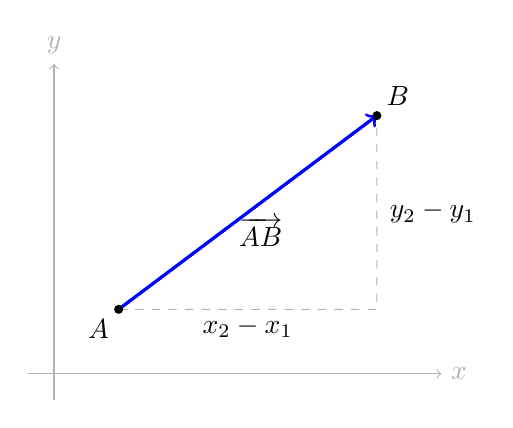
\begin{tikzpicture}[scale=0.82]
	\draw[->,gray!60] (-0.4,0) -- (6.0,0) node[right] {$x$};
	\draw[->,gray!60] (0,-0.4) -- (0,4.8) node[above] {$y$};
	\coordinate (A) at (1.0,1.0);
	\coordinate (B) at (5.0,4.0);
	\draw[dashed,gray!60] (A) -- (5.0,1.0) -- (B);
	\draw[very thick,blue,->] (A) -- (B);
	\fill (A) circle (2pt) node[below left] {$A$};
	\fill (B) circle (2pt) node[above right] {$B$};
	\node at (3.2,2.2) {$\overrightarrow{AB}$};
	\node at (3.0,0.72) {$x_2-x_1$};
	\node[right] at (5.05,2.5) {$y_2-y_1$};
\end{tikzpicture}
\end{center}
\textbf{途中式（代表例）}
\begin{align*}
&1.\ \overrightarrow{AB}=(5-1,\ 7-2)=(4,5),\ |\overrightarrow{AB}|=\sqrt{4^2+5^2}=\sqrt{41}\\
&6.\ \overrightarrow{AB}=(c-a,\ d-b),\ |\overrightarrow{AB}|=\sqrt{(c-a)^2+(d-b)^2}
\end{align*}

\newpage
\section{ベクトルの足し算・引き算・スカラー倍 解答}
\begin{align*}
&1.\ \begin{pmatrix}7 & 2\end{pmatrix}\\[0.45em]
&2.\ \begin{pmatrix}-5 & 9\end{pmatrix}\\[0.45em]
&3.\ \begin{pmatrix}6 & -10\end{pmatrix}\\[0.45em]
&4.\ \begin{pmatrix}6 & -12\end{pmatrix}\\[0.45em]
&5.\ \begin{pmatrix}-6 & 8\end{pmatrix}\\[0.45em]
&6.\ \begin{pmatrix}8 & -17\end{pmatrix}
\end{align*}
\textbf{考え方}\
足し算・引き算・スカラー倍は、各成分ごとにそのまま計算する。\\
\textbf{途中式（代表例）}
\begin{align*}
&5.\ \begin{pmatrix}1 & 2\end{pmatrix}+\begin{pmatrix}-3 & 5\end{pmatrix}-\begin{pmatrix}4 & -1\end{pmatrix}\\
&\quad =\begin{pmatrix}1-3-4 & 2+5+1\end{pmatrix}=\begin{pmatrix}-6 & 8\end{pmatrix}\\
&6.\ 2\vec{a}-3\vec{b}=2\begin{pmatrix}1 & -4\end{pmatrix}-3\begin{pmatrix}-2 & 3\end{pmatrix}\\
&\quad =\begin{pmatrix}2 & -8\end{pmatrix}+\begin{pmatrix}6 & -9\end{pmatrix}=\begin{pmatrix}8 & -17\end{pmatrix}
\end{align*}

\newpage
\section{内積と角度 解答}
\begin{align*}
&1.\ 11\\[0.45em]
&2.\ 0\\[0.45em]
&3.\ \text{垂直}\\[0.45em]
&4.\ \theta=\cos^{-1}\!\left(\frac45\right)\\[0.45em]
&5.\ \theta=60^\circ\\[0.45em]
&6.\ \vec{a}\cdot\vec{b}=0,\ \text{よって垂直}
\end{align*}
\textbf{考え方}\
内積は $\vec{a}\cdot\vec{b}=a_1b_1+a_2b_2$。0 なら垂直、角度は $\cos\theta=\dfrac{\vec{a}\cdot\vec{b}}{|\vec{a}||\vec{b}|}$ を使う。\\
	extbf{図説（内積と角度）}
\begin{center}
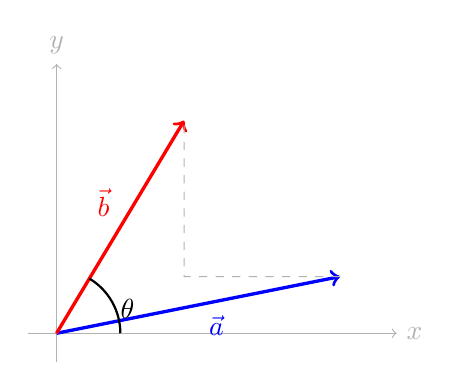
\begin{tikzpicture}[scale=0.9]
	\draw[->,gray!60] (-0.4,0) -- (4.8,0) node[right] {$x$};
	\draw[->,gray!60] (0,-0.4) -- (0,3.8) node[above] {$y$};
	\coordinate (O) at (0,0);
	\coordinate (A) at (4,0.8);
	\coordinate (B) at (1.8,3.0);
	\draw[very thick,blue,->] (O) -- (A) node[midway,below right] {$\vec{a}$};
	\draw[very thick,red,->] (O) -- (B) node[midway,above left] {$\vec{b}$};
	\draw[dashed,gray!60] (A) -- (1.8,0.8) -- (B);
	\draw[thick] (0.9,0) arc (0:59:0.9);
	\node at (1.0,0.35) {$\theta$};
\end{tikzpicture}
\end{center}
\textbf{途中式（代表例）}
\begin{align*}
&4.\ \vec{a}\cdot\vec{b}=2\cdot1+1\cdot2=4,\ |\vec{a}|=\sqrt5,\ |\vec{b}|=\sqrt5\\
&\quad \cos\theta=\frac{4}{\sqrt5\sqrt5}=\frac45\Rightarrow \theta=\cos^{-1}\!\left(\frac45\right)\\
&5.\ \vec{a}\cdot\vec{b}=4\cdot2+0\cdot2\sqrt3=8,\ |\vec{a}|=4,\ |\vec{b}|=4\\
&\quad \cos\theta=\frac{8}{4\cdot4}=\frac12\Rightarrow \theta=60^\circ
\end{align*}

\newpage
\section{2次元の外積と面積 解答}
\begin{align*}
&1.\ -5\\[0.45em]
&2.\ 13\\[0.45em]
&3.\ 12\\[0.45em]
&4.\ 12\\[0.45em]
&5.\ \vec{a}\times\vec{b}=-(\vec{b}\times\vec{a})\\[0.45em]
&6.\ \vec{a}\times\vec{b}=5,\ \vec{a}\times\vec{c}=-5
\end{align*}
\textbf{考え方}\
2次元の外積は $\vec{a}\times\vec{b}=a_xb_y-a_yb_x$ として計算する。平行四辺形の面積はその絶対値。\\
\textbf{途中式（代表例）}
\begin{align*}
&3.\ \begin{pmatrix}4 & 0\end{pmatrix}\times\begin{pmatrix}0 & 3\end{pmatrix}=4\cdot3-0\cdot0=12\\
&4.\ \text{面積}=|12|=12\\
&6.\ \vec{a}\times\vec{b}=2\cdot3-1\cdot1=5,\ \vec{a}\times\vec{c}=2\cdot(-1)-1\cdot3=-5
\end{align*}

\newpage
\section{射影とゲーム計算 解答}
\begin{align*}
&1.\ \begin{pmatrix}3 & 0\end{pmatrix}\\[0.45em]
&2.\ \begin{pmatrix}0 & 1\end{pmatrix}\\[0.45em]
&3.\ \begin{pmatrix}\frac95 & \frac{12}{5}\end{pmatrix}\\[0.45em]
&4.\ \text{当たらない}\\[0.45em]
&5.\ \begin{pmatrix}2 & 2\end{pmatrix}\\[0.45em]
&6.\ \begin{pmatrix}0 & -2\end{pmatrix}
\end{align*}
\textbf{考え方}\
単位ベクトル $\hat{b}$ 方向への射影は $\vec{a}\cdot\hat{b}$ を長さとして、$\left(\vec{a}\cdot\hat{b}\right)\hat{b}$ で求める。衝突判定は中心間距離と半径和を比べる。\\
\textbf{図説（射影）}
\begin{center}
\begin{tikzpicture}[scale=0.9]
	\draw[->,gray!60] (-0.4,0) -- (5.6,0) node[right] {$x$};
	\draw[->,gray!60] (0,-0.4) -- (0,3.8) node[above] {$y$};
	\coordinate (O) at (0,0);
	\coordinate (A) at (4.2,2.0);
	\coordinate (P) at (4.2,0);
	\draw[very thick,blue,->] (O) -- (A) node[midway,above left] {$\vec{a}$};
	\draw[very thick,red,->] (O) -- (5,0) node[midway,below] {$\hat{b}$};
	\draw[dashed,gray!60] (A) -- (P);
	\draw[very thick,green!60!black,->] (O) -- (P) node[midway,below] {$\vec{A}$};
	\fill (A) circle (2pt);
	\fill (P) circle (2pt);
\end{tikzpicture}
\end{center}
\textbf{途中式（代表例）}
\begin{align*}
&3.\ \vec{a}\cdot\hat{b}=\begin{pmatrix}5 & 0\end{pmatrix}\cdot\begin{pmatrix}\frac35 & \frac45\end{pmatrix}=3\\
&\quad \vec{A}=3\begin{pmatrix}\frac35 & \frac45\end{pmatrix}=\begin{pmatrix}\frac95 & \frac{12}{5}\end{pmatrix}\\
&4.\ |AB|=\sqrt{(5-2)^2+(3.6-2)^2}=\sqrt{11.56}=3.4,\ r_a+r_b=3.0\\
&\quad 3.4>3.0\Rightarrow\text{当たらない}\\
&5.\ \vec{v}\cdot\hat{w}=\begin{pmatrix}4 & 0\end{pmatrix}\cdot\begin{pmatrix}\frac1{\sqrt2} & \frac1{\sqrt2}\end{pmatrix}=2\sqrt2\\
&\quad \vec{v}_{\parallel}=2\sqrt2\begin{pmatrix}\frac1{\sqrt2} & \frac1{\sqrt2}\end{pmatrix}=\begin{pmatrix}2 & 2\end{pmatrix}
\end{align*}

\end{document}